\subsection{Űrlapok}

%86
\begin{frame}
  Vastag kliens alkalmazásokhoz hasonlóan adatok gyűjthetőek űrlapokkal, amiket 
  \begin{itemize}
    \item feldolgoztathatunk a szerver oldalon (most ez lesz), vagy
    \item JavaScript programmal a kliensen.
  \end{itemize}
  Űrlap vezérlők a \texttt{<form>} elembe ágyazva használhatók. Legfontosabb attribútumai:
  \begin{description}[m]
    \item[\texttt{action}] \hfill \\ A szerver oldali feldolgozó script URL-je
    \item[\texttt{target}] \hfill \\ Hova töltse a szerver válaszát 
    (\texttt{\_blank}, \texttt{\_self} (alapért.), \texttt{\_parent}, \dots)
    \item[\texttt{novalidate}] \hfill \\ Ne végezzen input 
    ellenőrzést a böngésző
    \item[\texttt{autocomplete}] \hfill \\ Korábban megadottak alapján 
    kiegészíti az adatokat (\texttt{on} (alapért.), \texttt{off})
  \end{description}
\end{frame}

%87
\begin{frame}
  \begin{description}[m]
    \item[\texttt{method}] \hfill \\ Adattovábbítási módszer:
    \begin{description}[m]
      \item[\texttt{get}] \hfill \\ Alapértelmezett. URL lekérdező 
      karakterláncában továbbítja az adatokat.
      \begin{itemize}
        \item Az URL betehető a könyvjelzők közé, és
        \item a böngészőben is könnyen szerkeszthető
      \end{itemize}
      \item[\texttt{post}] \hfill \\ HTTP tranzakcióként továbbít.
      \begin{itemize}
        \item Nincsenek méretkorlátok (URL hossza korlátozott, 
        $\approx$ 2000 karakter)
        \item Fájlok csak így továbbíthatók
        \item A böngészőben nem látszik, de ettől még \kiemel{nyílt 
        szöveg}ként továbbítják a hálózaton!
      \end{itemize}
    \end{description}
  \end{description}
\end{frame}

%88
\begin{frame}
  \begin{description}[m]
    \item[\texttt{enctype}] (type of encoding) \hfill \\ Meghatározza 
    a küldött adatok kódolását. Kötelező megadni, ha a \texttt{method} 
    attr. értéke \texttt{post}. Lehetséges értékek:
    \begin{description}[m]
      \item[\texttt{application/x-www-form-urlencoded}] \hfill \\ 
      Alapértelmezett. Minden szóközt és speciális karaktert 
      helyettesít.
      \item[\texttt{multipart/form-data}] \hfill \\ Fájlok küldésekor 
      kell használni.
      \item[\texttt{\texttt{text/plain}}] \hfill \\ Csak a szóközöket 
      helyettesíti.
    \end{description}
  \end{description}
\end{frame}

%89
\begin{frame}
  A legtöbb vezérlő az \texttt{<input>} elemmel hozható létre, pl. 
  egy számbeviteli mező néhány attribútuma, és hatása:
  \begin{description}[m]
    \footnotesize
    \item[\texttt{type}] \hfill \\ \texttt{number}, számbeviteli mező 
    létrehozása
    \item[\texttt{name}] \hfill \\ A szerver oldalon ez lesz az adat 
    \emph{kulcsa}
    \item[\texttt{min}] \hfill \\ A legkisebb bevihető érték
    \item[\texttt{max}] \hfill \\ A legnagyobb bevihető érték
    \item[\texttt{step}] \hfill \\ Ennyit változtatnak a 
    léptetőgombok/kurzurvezérlő nyilak az értéken, ennyi 
    többszöröseit lehet megadni, illetve ha 
    értéke \texttt{any}, akkor bármilyen racionális szám megadható
    \item[\texttt{required}] \hfill \\ A mező kitöltése kötelező
  \end{description}
\end{frame}

%90
\begin{frame}
  Űrlapbeküldő gomb: \texttt{<input>} elem
  \begin{itemize}
    \item \texttt{type="submit"}
    \item \texttt{value} attr. adja meg a gomb feliratát
  \end{itemize}
  \vfill
  Cimke létrehozása vezérlőhöz: \texttt{<label>} elemmel. A 
  cimkére kattintva a vezérlő is aktiválódik (pl. rádiógombnál 
  kiválasztás). Kapcsolat cimke és 
  vezérlő között:
  \begin{itemize}
    \item vezérlő a cimke belsejébe ágyazva
    \item a cimke \texttt{for} attribútumában megadható a vezérlő 
    \texttt{id}-je
  \end{itemize}
\end{frame}

%91
\begin{frame}
  Vezérlők logikai csoportosítása: \texttt{<fieldset>} elemmel\\
  Csoport feliratának megadása: \texttt{<legend>} elemben
  \vfill
  \begin{center}
    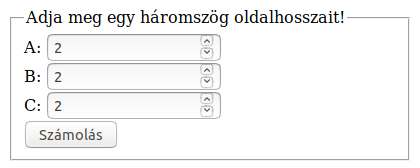
\includegraphics[width=.5\textwidth]{urlap1.png}
  \end{center}
\end{frame}

%92
\begin{frame}
  \begin{exampleblock}{\textattachfile{urlap1.html}{urlap1.html} 
  (\textattachfile{urlap1.php}{urlap1.php})}
    \footnotesize
    \lstinputlisting[style=HTML,linerange={8-20},numbers=left,firstnumber=8]{urlap1.html}
  \end{exampleblock}
\end{frame}

%93
\begin{frame}
  A legtöbb vezérlő az \texttt{<input>} elemmel és annak \texttt{type} 
  attribútumával állítható elő. Az összes vezérlővel használható főbb 
  attribútumai: 
  \begin{description}[m]
    \item[\texttt{autocomplete}] \hfill \\ Automatikus kiegészítés a 
    korábban begépelt tartalom alapján. (\texttt{on}, \texttt{off}) 
    \item[\texttt{autofocus}] \hfill \\ Oldalbetöltés után 
    automatikusan fókuszba kerül 
    \item[\texttt{disabled}] \hfill \\ Letiltott vezérlő 
    \item[\texttt{form}] \hfill \\ Ha a vezérlő 
    nincs \texttt{<form>} elembe ágyazva, akkor annak \texttt{id}-je 
    alapján logikailag összekapcsolható vele.
  \end{description}
\end{frame}

%94
\begin{frame}
  \begin{description}[m]
    \item[\texttt{id}] \hfill \\ A vezérlőt egyedileg azonosítja a 
    \kiemel{kliens} oldalon (pl. JavaScript programokban)
    \item[\texttt{name}] \hfill \\ A vezérlőt azonosítja a 
    \kiemel{szerver} oldalon (kulcs) 
    \item[\texttt{readonly}] \hfill \\ Csak olvashatóvá teszi a vezérlőt 
    \item[\texttt{required}] \hfill \\ A mező kitöltése kötelező 
    \item[\texttt{value}] \hfill \\ A vezérlő értéke
  \end{description}
\end{frame}

%95
\begin{frame}
  Egysoros szövegbeviteli mező: \texttt{type="text"} (alapértelmezés)
  \begin{description}[m]
    \item[\texttt{list}] \hfill \\ Egy \texttt{<datalist>} elem (ajánlatok legördülő listája) \texttt{id}-jét tartalmazza
    \item[\texttt{maxlength}] \hfill \\ A begépelhető karakterek száma
    \item[\texttt{pattern}] \hfill \\ Reguláris kifejezés az érték ellenőrzéséhez. Hiba esetén a \texttt{title} értéke magyarázza az elvárt formátumot.
    \item[\texttt{placeholder}] \hfill \\ Helyőrző, ami az első karakter begépeléséig segít a felhasználónak, pl. ,,A rendszámot kötőjel nélkül, nagybetűkkel adja meg!''
    \item[\texttt{size}] \hfill \\ A vezérlő szélessége átlagos karakterszélességben mérve (CSS jobb)
  \end{description}
\end{frame}

%96
\begin{frame}
  A \texttt{<datalist>} elembe \texttt{<option>} elemek ágyazhatók, 
  melyek gépelést segítő legördülő lista elemeiként jelennek meg.\\
  A (\texttt{<select>} elemben is használható) \texttt{<option>} attribútumai:
  \begin{description}[m]
    \item[\emph{attribútum nélkül}] \hfill \\ Az elem tartalma jelenik meg a legördülő listában, és ezt továbbítják a szervernek is
    \item[\texttt{label}] \hfill \\ A listában egy rövidebb szöveg jelenhet meg, mint az elem értéke
    \item[\texttt{selected}] \hfill \\ Kiválasztottá teszi az elemet az oldal betöltésekor (csak \texttt{<select>-nél})
    \item[\texttt{value}] \hfill \\ Ha megadják, ennek tartalmát küldi a szervernek (vagy másolja a szövegmezőbe), nem a megjelenő szöveget
  \end{description}
\end{frame}

%97
\begin{frame}
  Reguláris kifejezések dióhéjban\\
  \vfill
  Általános forma: \texttt{/\kiemel{minta}/módosítók}\\
  Input ellenőrzésre csak a \texttt{minta} szolgál; ha a vezérlő értéke nem illeszkedik az általános mintára, az űrlapot nem lehet beküldeni.\\
  \begin{itemize}
    \item Az általános karakterek önmagukat reprezentálják.
    \item A metakarakterek önmagukban is halmazt vagy vezérlőjelet testesítenek meg, pl. \texttt{\textbackslash d} a számjegyek, \texttt{\textbackslash s} a fehér karakterek, \texttt{\textbackslash n} az újsor, stb.
    \item Halmaz elemei közül elég egynek illeszkednie, pl. \texttt{[abc]} elfogadja az abc első három betűje közül bármelyiket.
    \item Halmaz intervallummal is megadható, pl. \texttt{[a-z]} a kisbetűk halmaza, de a két módszer kombinálható is, pl. \texttt{[a-zA-Z]} a betűk halmaza.
    \item Az \texttt{[\textasciicircum abc]} minden jelre illeszkedik, ami nem \texttt{a}, \texttt{b}, és \texttt{c}.
    \item Alternatívák is létrehozhatók \texttt{(a|b)} formában.
  \end{itemize}  
\end{frame}

%98
\begin{frame}
  Mennyiségek szabályozása
  \medskip
  \begin{itemize}
    \item \texttt{n+} legalább egy előfordulást vár el
    \item \texttt{n*} 0 vagy több előfordulást követel
    \item \texttt{n?} 0 vagy 1 előfordulás
    \item \texttt{n\{X\}} pontosan X előfordulás
    \item \texttt{n\{X,Y\}} legalább X, legfeljebb Y előfordulás
    \item \texttt{n\{X,\}} legalább X előfordulás
  \end{itemize}
  Pl. egy rendszámot ellenőriz a \texttt{[A-Za-z]\{3\}-\textbackslash d\{3\}} minta. 
  \hiv{\href{http://html5pattern.com/}{További minták.}}
  \vfill
  \hiv{\href{https://developer.mozilla.org/en-US/docs/Web/JavaScript/Guide/Regular_Expressions}{További részletek}}
\end{frame}

%99
\begin{frame}
  \begin{center}
    
\includegraphics[width=.5\textwidth]{urlap2-1.png}\\\vspace{-.5cm}\hrulefill\\
    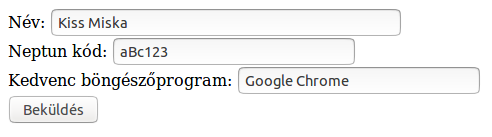
\includegraphics[width=.5\textwidth]{urlap2-2.png}\\\vspace{-.5cm}\hrulefill\\
    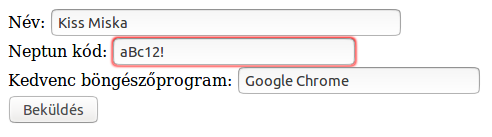
\includegraphics[width=.5\textwidth]{urlap2-3.png}\\
  \end{center}
\end{frame}

%100
\begin{frame}
  \begin{exampleblock}{\textattachfile{urlap2.html}{urlap2.html} (\textattachfile{urlap2.php}{urlap2.php})}
    \footnotesize
    \lstinputlisting[style=HTML,linerange={9-15},numbers=left,firstnumber=9]{urlap2.html}
  \end{exampleblock}
\end{frame}

%101
\begin{frame}
  \begin{exampleblock}{\textattachfile{urlap2.html}{urlap2.html} (\textattachfile{urlap2.php}{urlap2.php})}
    \footnotesize
    \lstinputlisting[style=HTML,linerange={16-25},numbers=left,firstnumber=16]{urlap2.html}
  \end{exampleblock}
\end{frame}

%102
\begin{frame}
  Jelszóbeviteli mező: \texttt{type="password"}\\
  Nagyon hasonló a \texttt{text} típushoz, de a karaktereket ,,elrejti'' (viszont \kiemel{nem titkosítja}!)
  \vfill
  Színválasztó: \texttt{type="color"}\\
  A \texttt{value} értéke \texttt{\#RRGGBB} formátumú.
  \vfill
  Dátumválasztó: \texttt{type="date"}\\
  A \texttt{value} értéke \emph{éééé-hh-nn} formátumú. Használhatóak még a \texttt{min}, \texttt{max} attribútumok.
  \vfill
  Dátum és időválasztó (időzóna nélkül):  \texttt{type="datetime-local"}\\
  A \texttt{value} értéke \emph{éééé-hh-nnTóó:pp} formátumú.
\end{frame}

%103
\begin{frame}
  E-mail cím megadása: \texttt{type="email"}\\
  Automatikusan ellenőrzi formailag. Több cím is megadható vesszőkkel elválasztva, ha megadják a \texttt{multiple} attribútumot.
  \vfill
  Rejtett mező: \texttt{type="hidden"}\\
  Egyáltalán nem jelenik meg, de egy (pl. JavaScript kóddal előállított) kulcs 
  (\texttt{name}) - érték (\texttt{value}) pár felküldhető a szerverre.
  \vfill
  Fájlok feltöltése: \texttt{type="file"}\\
  Több fájl feltölthető a \texttt{multiple} attribútum megadásával. 
  Korlátozható a tallózható fájlok köre, pl. \texttt{accept=".jpg"} csak 
  JPEG fájlokat enged, egy MIME-típus, mint pl. a \texttt{accept="video/*"} 
  mindenféle videót, stb. Korlátozható a fájlok mérete is:\\
  \texttt{<input type="hidden" name="MAX\_FILE\_SIZE" value="\emph{méret}" />}\\
  A kódolás típusa legyen \texttt{enctype="multipart/form-data"}, a HTTP 
  metódus \texttt{method="POST"}!
\end{frame}

%104
\begin{frame}
  \begin{center}
    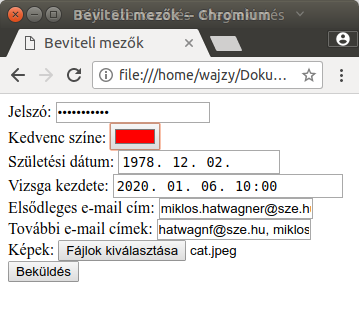
\includegraphics[width=.5\textwidth]{urlap3.png}
  \end{center}
\end{frame}

%105
\begin{frame}
  \begin{exampleblock}{\textattachfile{urlap3.html}{urlap3.html} (\textattachfile{urlap3.php}{urlap3.php})}
    \footnotesize
    \lstinputlisting[style=HTML,linerange={8-17},numbers=left,firstnumber=8]{urlap3.html}
  \end{exampleblock}
\end{frame}

%106
\begin{frame}
  \begin{exampleblock}{\textattachfile{urlap3.html}{urlap3.html} (\textattachfile{urlap3.php}{urlap3.php})}
    \footnotesize
    \lstinputlisting[style=HTML,linerange={18-27},numbers=left,firstnumber=18]{urlap3.html}
  \end{exampleblock}
\end{frame}

%107
\begin{frame}
  \begin{exampleblock}{Készítse el az alábbi űrlapot! (\textattachfile{urlap4.html}{urlap4.html})}
    Az adatokat küldje a \texttt{http://xenia.sze.hu/\textasciitilde wajzy/html/urlap3.php} címre!
    \begin{columns}[T]
      \column{0.45\textwidth}
        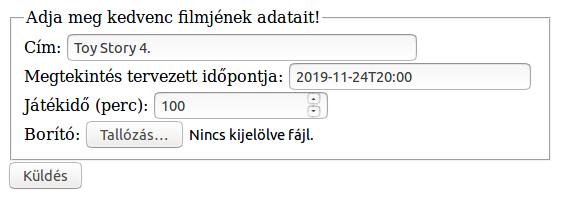
\includegraphics[width=\textwidth]{urlap4-1.png}
      \column{0.45\textwidth}
        
\includegraphics[width=\textwidth]{urlap4-2.png}
    \end{columns} 
  \end{exampleblock}
\end{frame}

%108
\begin{frame}
  Év és hónap kiválasztás: \texttt{type="month"}\\
  A \texttt{value} értéke \emph{éééé-hh} formátumú. Használhatóak még a \texttt{min}, \texttt{max} attribútumok.
  \vfill
  Év és azon belül egy hét kiválasztása: \texttt{type="week"}\\
  A \texttt{value} értéke \emph{éééé-Whh} formátumú.
  \vfill
  Idő megadása: \texttt{type="time"}\\
  A \texttt{value} értéke \emph{óó:pp} formátumú.
  \vfill
  Nyomógomb: \texttt{type="button"}\\
  Önmagában semmire nem jó, JavaScript kódok futtatására használják.
  \vfill
  Űrlap alaphelyzetbe állítása: \texttt{type="reset"}\\
  Az űrlap betöltése utáni állapotot állítja vissza; ha véletlenül kattintanak rá, minden addigi munka elvész!
\end{frame}

%109
\begin{frame}
  Jelölőnégyzet: \texttt{type="checkbox"}\\
  Egymástól független választási lehetőségekhez. 
  \vfill
  Rádiógomb: \texttt{type="radio"}\\
  Egy rádiógomb-csoporton belül csak egy elem lehet kiválasztva. 
  A felhasználó nem tudja az összes elemet ki nem választottá 
  tenni. Csoportképző módszer: azonos \texttt{name} attribútum 
  értékek.
  \vfill
  Mindkét típusra igaz, hogy egy elemet kiválasztani a 
  \texttt{checked} attribútummal lehet. A \texttt{value} attribútumot rádiógomboknál 
  ,,kötelező'' megadni, mert különben csak az \texttt{on} értéket 
  kapja meg a szerver $\to$ a gomb azonosíthatatlan. A ki nem 
  választott elemeknek még a kulcsa sem látszik a szerveren.
\end{frame}

%110
\begin{frame}
  \begin{center}
    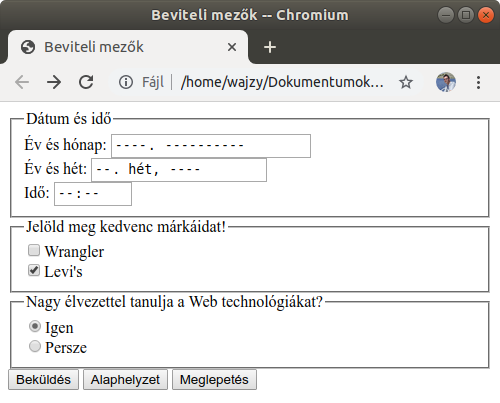
\includegraphics[width=.5\textwidth]{urlap5.png}
  \end{center}
\end{frame}

%111
\begin{frame}
  \begin{exampleblock}{\textattachfile{urlap5.html}{urlap5.html}}
    \footnotesize
    \lstinputlisting[style=HTML,linerange={11-16},numbers=left,firstnumber=11]{urlap5.html}
    \lstinputlisting[style=HTML,linerange={19-23},numbers=left,firstnumber=19]{urlap5.html}
  \end{exampleblock}
\end{frame}

%112
\begin{frame}
  \begin{exampleblock}{\textattachfile{urlap5.html}{urlap5.html}}
    \footnotesize
    \lstinputlisting[style=HTML,linerange={27-30},numbers=left,firstnumber=27]{urlap5.html}
    \lstinputlisting[style=HTML,linerange={34-35},numbers=left,firstnumber=34]{urlap5.html}
  \end{exampleblock}
\end{frame}

%113
\begin{frame}
  Beküldés gomb képpel helyettesítve: \texttt{type="image"}\\
  \texttt{src}  adja meg a képet, \texttt{width} a szélességet, 
  \texttt{height} a magasságot, \texttt{alt} a helyettesítő 
  szöveget. Beküldi a kattintás helyét is (\texttt{x}, \texttt{y} 
  kulcsok).
  \vfill
  A \texttt{submit} és \texttt{image} vezérlők néhány közös 
  attribútuma:
  \begin{itemize}
    \item \texttt{formaction}: a \texttt{<form>} \texttt{action} 
    attribútumának értékét írja felül; pl. két gomb két 
    külön helyre küldheti az adatokat.
    \item \texttt{formenctype}, \texttt{formmethod}, 
    \texttt{formnovalidate}, \texttt{formtarget} hasonlóan, a 
    \texttt{<form>} attribútum értékeinek felülírására szolgál.
  \end{itemize}
\end{frame}

%114
\begin{frame}
  Csúszka: \texttt{type="range"}\\
  Alapértelmezetten [0, 100] közti érték kiválasztására, ahol a 
  pontos érték nem számít. Adatbevitel szabályozható a 
  \texttt{min}, \texttt{max}, \texttt{step} attribútumokkal.
  \vfill
  Keresőmező: \texttt{type="search"}\\
  Adatok keresésére egy oldalon.
  \vfill
  Telefonszám: \texttt{type="tel"}\\
  A bevitt szám ellenőrizhető a \texttt{pattern} segítségével.
  \vfill
  URL: \texttt{type="url"}\\
  A böngésző formai ellenőrzést végezhet vagy speciális gombokat 
  tehet a virtuális billentyűzetre (pl. \emph{.com}, \emph{www.}, \dots)
\end{frame}

%115
\begin{frame}
  \begin{columns}[T]
    \column{0.3\textwidth}
      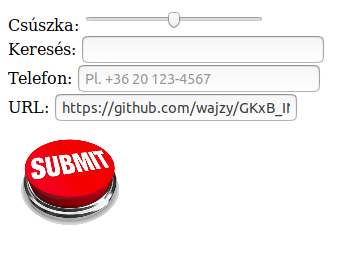
\includegraphics[width=\textwidth]{urlap6-1.png}
    \column{0.66\textwidth}
      
\includegraphics[width=\textwidth]{urlap6-2.png}
  \end{columns}
\end{frame}

%116
\begin{frame}
  \begin{exampleblock}{\textattachfile{urlap6.html}{urlap6.html} 
  (\textattachfile{urlap6-submit.png}{urlap6-submit.png}, \textattachfile{urlap2.php}{urlap2.php})}
    \footnotesize
    \lstinputlisting[style=HTML,linerange={9-22},numbers=left,firstnumber=9]{urlap6.html}
  \end{exampleblock}
\end{frame}

%117
\begin{frame}
  Vezérlők, amiket \emph{nem} az \texttt{input} elemmel hozunk létre:
  \begin{description}[m]
    \item[\texttt{<select>}] \hfill \\ Legördülő lista, melynek 
    bejegyzéseit \texttt{option} elemekkel adhatjuk meg. Attribútumai:
    \begin{description}[m]
      \item[\texttt{size}] \hfill \\ Ennyi elem fog látszani egyszerre 
      egymás alatt (görgethető doboz)
      \item[\texttt{multiple}] \hfill \\ Több elem is kiválasztható 
      egyszerre (Ctrl, Shift) (PHP: a \texttt{name} értéke 
      \texttt{[]}-re végződjön!)
    \end{description}
    \item[\texttt{<optgroup>}] \hfill \\ Sok lehetőség esetén 
    csoportok képzésére: \texttt{<select>} $\to$ \texttt{<optgroup>} 
    $\to$ \texttt{<option>}
    \begin{description}[m]
      \item[\texttt{label}] \hfill \\ Csoport (ki nem választható) 
      felirata
    \end{description}
  \end{description}
\end{frame}

%118
\begin{frame}
  \begin{description}[m]
    \item[\texttt{<textarea>}] \hfill \\ Hosszabb szövegek 
    megadására. Még a címkék közötti fehér karaktereket is 
    belefoglalja a vezérlő tartalmába! Attribútumok:
    \begin{description}[m]
      \item[rows] \hfill \\ Sorok száma
      \item[cols] \hfill \\ Oszlopok száma
    \end{description}
    \item[<button>] \hfill \\ Hasonló, mint \texttt{<input 
    type="button">}, de HTML/CSS formázható tartalommal.
    \begin{description}[m]
      \item[type] \hfill \\ A gomb típusa, lehet \texttt{button}, 
      \texttt{submit} és \texttt{reset}.
    \end{description}
  \end{description}
\end{frame}

%119
\begin{frame}
  \begin{description}[m]
    \item[\texttt{<output>}] \hfill \\ JavaScript számítások 
    eredményének jelölésére. Nincs látványos formázása.
    \begin{description}[m]
      \item[\texttt{for}] \hfill \\ Azon \texttt{<input>} elemek 
      \texttt{id}-i szóközzel elválasztva, melyekből kiindulva az eredmény 
      megszületett.
    \end{description}
  \end{description}
  \begin{columns}[T]
    \column{0.5\textwidth}
      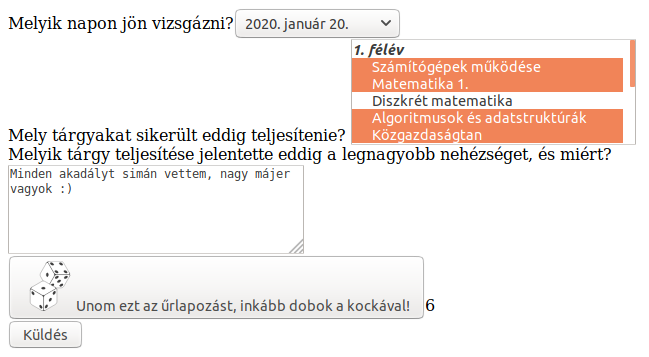
\includegraphics[width=\textwidth]{urlap7-1.png}
    \column{0.45\textwidth}
      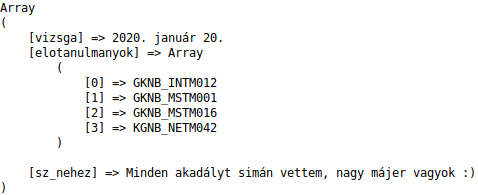
\includegraphics[width=\textwidth]{urlap7-2.png}
  \end{columns}
\end{frame}

%120
\begin{frame}
  \begin{exampleblock}{\textattachfile{urlap7.html}{urlap7.html} 
  (\textattachfile{dice.svg}{dice.svg}, \textattachfile{urlap2.php}{urlap2.php})}
    \footnotesize
    \lstinputlisting[style=HTML,linerange={9-14},numbers=left,firstnumber=9]{urlap7.html}
  \end{exampleblock}
\end{frame}

%121
\begin{frame}
  \begin{exampleblock}{\textattachfile{urlap7.html}{urlap7.html}}
    \footnotesize
    \lstinputlisting[style=HTML,linerange={15-18},numbers=left,firstnumber=15]{urlap7.html}
    \lstinputlisting[style=HTML,linerange={22-25},numbers=left,firstnumber=22]{urlap7.html}
    \lstinputlisting[style=HTML,linerange={29-31},numbers=left,firstnumber=29]{urlap7.html}
  \end{exampleblock}
\end{frame}

%122
\begin{frame}
  \begin{exampleblock}{\textattachfile{urlap7.html}{urlap7.html}}
    \footnotesize
    \lstinputlisting[style=HTML,linerange={32-40},numbers=left,firstnumber=32]{urlap7.html}
  \end{exampleblock}
\end{frame}

%123
\begin{frame}
  \scriptsize
  A mellékelt ábrának megfelelően hozzon létre egy weboldalt! Az adatokat küldje a \texttt{http://xenia.sze.hu/\textasciitilde wajzy/html/urlap2.php} címre!
  \begin{columns}[c]
    \column{0.25\textwidth}
      \begin{itemize}
        \item Az \emph{Extrák} közül többet is lehessen választani!
        \item A választható \emph{színek} legyenek: \emph{fehér}, \emph{szürke}, 
        \emph{fekete}, \emph{vörös}, \emph{kék}, \emph{sárga}. Alapértelmezetten legyen 
        kiválasztva a \emph{vörös}!
        \item A \emph{fényezés} típusa alapértelmezetten legyen 
        \emph{normál}!
      \end{itemize}
    \column{0.8\textwidth}
      \begin{exampleblock}{\small \textattachfile{urlap8.html}{urlap8.html}}
        \vspace{-.5cm}
        \begin{columns}[T]
          \column{0.45\textwidth}
            \begin{center}
              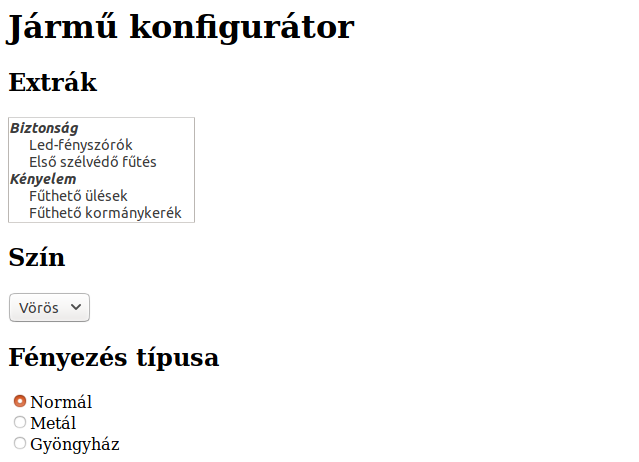
\includegraphics[width=\textwidth]{urlap8-1.png}\\
              \tiny Az oldal teteje
            \end{center}
          \column{0.45\textwidth}
            \begin{center}
              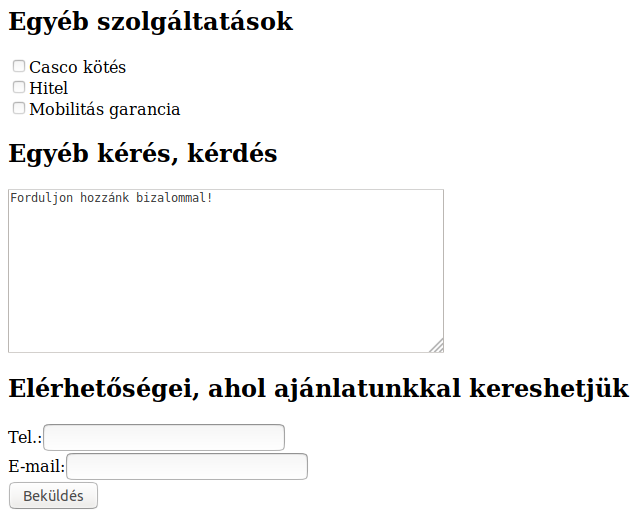
\includegraphics[width=\textwidth]{urlap8-2.png}\\
              \tiny Az oldal alja
            \end{center}
        \end{columns}
      \end{exampleblock}
  \end{columns}
\end{frame}
